\documentclass{article}

\usepackage{color}
\usepackage[utf8]{inputenc}
\usepackage{amsmath,textcomp,amssymb,geometry,graphicx,enumerate}
\usepackage[linesnumbered, ruled, noend ]{algorithm2e}
\usepackage{hyperref}       % hyperlinks
\hypersetup{
    colorlinks=true,
    linkcolor=blue,
    filecolor=magenta,      
    citecolor=blue,
    urlcolor=blue, %cyan
}

\frenchspacing

\title{Scaling Deep Learning with Actors and Asynchronous Tasks}
\author{Eric Liang, Richard Liaw, Zongheng Yang}
\date{May 2018}

\begin{document}

\maketitle
% \section {TODO}

% {\color{red} 

% (1) Practical content/creativity; implementation/tuning effort

% (2) Experimental data: scaling/performance analysis/interesting inputs or outputs

% (3) Theoretic content/creativity; design/analysis of algorithms

% (4) Impact: difficulty and timeliness of the contribution

% We understand that not all projects will have all four components but it is expected that the first two components will be present in all projects. As such, we expect the majority of your final report to be about parallelism, and not the problem description. }

\section{Introduction}
This project investigates supporting distributed deep learning training, using \textit{actors} and \textit{asynchronous tasks}, two programming models that are not commonly employed in these workloads.  In contrast, many state-of-the-art deep learning systems nowadays adopt the single-program, multiple-data (SPMD) programming model---examples include Distributed TensorFlow~\cite{tensorflow-osdi16} and Horovod~\cite{horovod}.  Qualitatively, decades of conventional wisdom in message-passing frameworks suggests that the SPMD paradigm is harder to program and debug yet can be highly efficient (e.g., MPI~\cite{MPI}).  Through this project, we show that a much more flexible and high-level programming model, based on tasks and actors, is able to match the performance of these specialized systems in neural network distributed training.  Key to our solution is making use of classical techniques seen in HPC and computer systems, such as maximizing the pipelining between computation and communication.

{\bf Problem setup.} For the remainder of the paper, we constrain the problem setting to neural network (NN) training using multiple machines each equipped with multiple GPUs.  All experiments consider the image classification model, \texttt{ResNet101}~\cite{resnet}, on synthetic dataset with the same format as ImageNet~\cite{imagenet}.  The key performance metric is \textit{throughput}, or total images processed (i.e., a forward and a corresponding backward pass have been performed) per second.

\subsection{Parallelism in Distributed Deep Learning}
Distributed deep learning originated as parameter servers ~\cite{param-server}, which are centralized and have state that is updated asynchronously among workers. With this lack of coordination comes a price - the inability to scale infinitely due to process noise introduced by the asynchrony.

Recent work has moved towards using synchronous updates for SGD as seen in Horovod~\cite{horovod}, utilizing a variety of high performance computing techniques (ie, allreduce) along with novel parameter tuning to come up with new implementations of SGD to use both more machines and achieve faster learning.

For a more complete treatment of different forms of parallelisms in deep learning, we refer the reader to the survey by Ben-Nun et al.~\cite{ben-nun18_demys_paral_distr_deep_learn}.

\subsection{Parallelisms via Actors and Tasks}
We implement all experiments in Ray~\cite{ray}, a new distributed execution engine that supports \textit{actors} and \textit{tasks}.  This section briefly describes the two constructs and how they specifically relate to distributed SGD.
Table~\ref{table:tasks-vs-actors} summarizes the properties of tasks and actors. 

\begin{table}[tbh]
\begin{center}
\begin{footnotesize}
\begin{tabular}{| c | c |}\hline
{\bf Tasks (stateless)} & {\bf Actors (stateful)} \\\hline
    Fine-grained load balancing & Coarse-grained load balancing \\\hline
    Support for object locality & Poor locality support \\\hline
    High overhead for small updates & Low overhead for small updates \\\hline
    Efficient failure handling & Overhead from checkpointing \\\hline
    % Application & light-weight simulations, & training, 3rd party \\
    %  examples   & input pre-processing  & stateful simulators \\\hline
\end{tabular}
\end{footnotesize}
\end{center}
\vspace{-0.6cm}
    \caption{\small{Tasks vs. actors tradeoffs.}}
\label{table:tasks-vs-actors}
\end{table}

{\bf Actors.} An \emph{actor} is a stateful (Python) process. Each actor exposes methods that
%is a stateful process that exposes a set
can be invoked remotely and are executed serially.
A method execution is similar to a task, in that it executes remotely and returns a future, but differs in that it executes on
a {\em stateful} worker. A {\em handle} to an actor can be passed to other actors or
tasks, making it possible for them to invoke methods on that actor.  

% \noindent {\bf How actors are used.}  
\textit{How actors are used in SGD.}
Naturally, we create several instances of \texttt{ParameterServerActor}, whose state is the NN parameters.  Additionally, SGD workers --- whose role is to calculate the forward/backward pass of an input batch --- are also expressed as actors, \texttt{SgdActor}.

{\bf Tasks.} A \emph{task} represents the execution of a remote
function on a stateless worker. When a remote function is invoked, a \emph{future}
representing the result of the task is returned immediately. Futures can be
retrieved using ${\bf ray.get()}$ and passed as arguments into other remote
functions without waiting for their result. This allows the user to express
parallelism while capturing data dependencies. 

\textit{How tasks are used in SGD.}
{\color{red} TODO}

{\color{red} TODO: maybe show pseudocode of the SgdActor/PsActor. Currently this discussion is pretty abstract w.r.t. SGD.}

% Remote functions operate on immutable objects and are expected to be
% \emph{stateless} and side-effect free: their outputs are determined solely by
% their inputs. This implies idempotence, which simplifies fault tolerance through function re-execution on failure.

% Tasks enable fine-grained load balancing through
% leveraging load-aware scheduling at task granularity, input data locality, as each task can be scheduled on the node storing its inputs, and low recovery overhead, as there is no need to checkpoint and recover intermediate state. In contrast, actors provide much more efficient fine-grained updates, as these updates are performed on internal rather than external state, which typically requires serialization and deserialization. For example, actors can be used to implement parameter servers~\citep{param-server} and GPU-based iterative computations (e.g., training). In addition, actors can be used to wrap third-party simulators and other opaque handles that are hard to serialize.
.....
\section{Exploring Distributed TensorFlow and Horovod}
Horovod is an implementation of allreduce distributed SGD using NCCL2 across machines and NCCL on . The algorithm is roughly as follows:

\textbf{Pseudocode.}
\begin{algorithm}
\caption{All-Reduce SGD}
\KwData{Input Data}
\For{all Nodes (simultaneously)} {
\For{all GPUs (simultaneously)}{
	instantiate data\;
	instantiate model replica\;
}
}
Barrier\;

\For{all Nodes (simultaneously)} {
\For{all GPUs (simultaneously)}{
	compute gradient based on data\;
	allreduce(gradient)\;
}
}


\For{all Nodes (simultaneously)} {
\For{all GPUs (simultaneously)}{
	apply gradient to model\;
}
}
\end{algorithm}

Distributed TensorFlow offers a variety of different distributed SGD implementations. For benchmarking we use a synchronized parameter server to reduce across nodes and an averaging scheme within node across GPUs. The algorithm is roughly as follows:

\textbf{Pseudocode.}
\begin{algorithm}
\caption{Synchronous Parameter Server SGD}
\KwData{Input Data, K Nodes}
\For{all Nodes (simultaneously)} {
\For{all GPUs (simultaneously)}{
	instantiate data\;
	instantiate model replica\;
}
}
generate N parameter server shards\;
\For{each shard in the N shards} {
    start parameter server on a different node \;
}
Barrier\;
\For{all Nodes (simultaneously)} {
\For{all GPUs (simultaneously)}{
	compute gradient based on data\;
	allreduce(gradient) on node\;
}
send shard of gradient to corresponding parameter server \;
wait for aggregated gradient \;
apply gradient to model \;
}
\For{all Parameter servers (simultaneously)}{
    \While {number of gradient shards $<$ K\;}{
        wait for gradient shard\;
    }
    
    aggregate all gradients\;
    broadcast gradients back to workers\;
}
\end{algorithm}

Note that in both cases, the amount of data transferred is constant \textit{per node} and is equal to $2 * N$, where $N$ is the size of the gradient. The total amount of bandwidth consumed scales linearly with the number of nodes.

To understand this, consider ring reduce. For $k$ participants, the gradient buffer is split into $k$ pieces, and each nodes sends and receives $N / k$ bytes over $k$ rounds. In total this means each node sends and receives $2 * N$ bytes.

A similar accounting holds for the parameter server. Each gradient produce must send $N$ bytes to the parameter server, and receive $N$ bytes from the parameter server. If the gradient is sharded into $k$ shards, then the network usage can be balanced evenly across all machines.

The main tradeoff between the ring reduce and shareded parameter server approach then, is the communication pattern itself. The parameter server requires all-to-all network communication, while ring reduce only requires neighboring nodes to communicate. However at the scales we are dealing with (up to 16 nodes), this is unlikely to be a bottleneck.

\section{Implementation and Optimizations}
In order to be achieve competitive levels of throughput, we had to utilize low-level primitives and write custom operators to avoid redundant copies and pipeline stages of the computation. All of our experiments used a Res-Net 101 model consisting of 168 MB of parameter weights. A standard forward pass with 64 images is roughly 40 ms.

\subsection{Memory Transfer between TensorFlow and Ray}
The compute engine, TensorFlow, manages all tensor memory buffers within a node.  To communicate tensors (gradients, in the case of SGD) across nodes, we make use of Ray's \textit{distributed object store} component (named Plasma).  Hence, memory transfer must happen between TensorFlow and Ray.

The strawman approach is straightforward.  With \texttt{gradients = sess.run(compute\_op)}, one asks TensorFlow to run calculation and returns a newly allocated \texttt{numpy.ndarray} that resides on host memory.  Then, one could perform \texttt{object\_id = ray.put(gradients)}, which amounts to a host-to-host memory copy---from ndarray to Ray's object store.  The remote nodes can subsequently fetch this object via \texttt{ray.get(object\_id)}.  In total there are three copies: (1) device memory to host memory (\texttt{tf.Tensor} to \texttt{np.ndarray}), (2) host memory to host memory (ndarray to Ray's object store), then (3) across-node communication.

We improve upon the strawman by eliminating the three copies down to two, the minimum necessary amount, by circumventing numpy completely.  The approach is to insert two custom TensorFlow operators into the dataflow graph.  The \texttt{TensorToPlasma} op schedules \texttt{cudaMemcpy} directly from \texttt{tf.Tensor} device memory to Plasma host memory, eliminating the unnecessary \texttt{np.ndarray} buffer.  The \texttt{PlasmaToTensor} op assumes the reversed role, copying from Plasma host memory into TensorFlow on-device buffers.  

To avoid stalling TensorFlow's compute, both ops create their own CUDA streams and launch the copy kernels onto their respective streams.  The host memory buffers are allocated and owned by Plasma, hence care has been taken to call CUDA's \texttt{cuMemHostRegister()} on those source/destination buffers; without such explicit registration, we observed that our custom copy ops stall the main compute stream, due to CUDA's ``default stream semantics''.  Lastly, to adhere to TensorFlow's dataflow semantics, care is taken to have our own copy streams properly synchronize on TensorFlow's compute stream, which makes sure any Tensor to copy has indeed been filled in by its upstream producer.

The above discussion assumes Tensor buffers reside on GPUs.  For CPU-owned Tensors, the strategy is to launch several threads that perform \texttt{memcpy()} on equal-sized chunks.  We note that this is a niche use case for deep learning users.

\subsection{Pipelining Computation with Communication}
{\color{red} ETC ETC.  We need to say the pipelining optimization is at the Ray level / or for across-node}.

We emphasize that, the above pipelining optimization is performed at the Ray level.  TensorFlow, the compute engine that launches CUDA kernels onto the GPUs, has implemented such pipelining at the device level.  Specifically, it uses at least 3 CUDA streams to dispatch kernels: a main stream for compute, a host-to-device copy stream, and a device-to-host copy stream.  Therefore, within a device, the communication and computation are already pipelined (up to black-box constraints imposed by the hardware).

\subsection{Gradient packing}
One key ingredient in enabling high performance was packing gradients. Gradient packing occurs after gradient calculation begins, and merges different size arrays from different layers into larger contiguous chunks. These chunks would later on be deconstructed back into the original tensor shapes in order to be applied to the model weights. 

This enabled a couple different minor optimizations. First, it amortized the memory transfer overhead from GPU to Ray's shared memory object store, maximizing throughput. It also was necessary to efficiently saturate the network. On the other hand, the size of the gradient packed could not be too large, as the receiving node would oversaturate, causing an overall slower implementation. In our experiments, we pack into roughly 10MB chunks, resulting in 15 chunks.

\subsection{Parameter Server Sharding and Placement}
Instead of using a centralized parameter server, we would shard the original model weights into distinct sections. The placement of these shards was important, as misplacement could reduce bandwidth. In our implementation, we make sure all parameter server shards are evenly placed on the nodes. 


\subsection{Scalability Bottlenecks}
\subsubsection{Network Bandwidth}


\subsubsection{Ring reduce + Fully utilizing GPUs on each machine}
The AWS p3.16xlarge instances have 8 GPUs, but surprisingly, it is not necessarily the case that more GPUs on a machine will scale better. We found for our scheme, using 4 GPUs per machine provided better scaling per GPU. We refer readers to the chart section below for a m

On the other hand For a single machine, ring reduce will outperform other methods. However, as we increase the number of machines, thek benefit of ring reduce is overshadowed by the network transfer overhead.

\section{Evaluation}
All experiments were run on Amazon EC2 using the p3.16xlarge instances.  Each instance has 8 Tesla V100 GPUs with 25Gbps Eternet bandwidth.  When possible, we launched instances in a placement group for faster inter-node network connection.  We conducted the following experiments:

\begin{enumerate}
    \item An end-to-end macrobencmark measuring training througput, for all three systems, utilizing up to 16 distinct instances (Figure~\ref{fig:sgd}).
    \item A microbenchmark that investigates a key limitation of our implementation: that using 8 GPUs per node yields worse scaling than using 4 GPUs per node, keeping the total number of GPUs constant (Figure~\ref{fig:8-vs-4-gpu}).
    \item A microbenchmark that investigates the best all-reduce strategies to use, within a node (Figure~\ref{fig:intra-node-allreduce-strategy}). 
\end{enumerate}

% \subsection{Single-Node Multi GPU SGD}
% Here we discuss some findings on Multi-GPU 
% \subsection{Charts}

\subsection{Macrobenchmark}
Figure~\ref{fig:sgd} shows the training throughput on ResNet-101 for three systems, Horovod, Distributed TensorFlow, and Ray (codenamed ``Halo'' in the graph).  In summary, our implementation in Ray is able to match Horovod and comes within 10\% of Distributed TensorFlow.  This result validates our hypothesis that the higher-level actor/task abstractions are able to match the SPMD/message-passing abstractions.

{\bf Weak Scaling.}  We note that the weak scaling factors, with 4 GPUs as baseline and with $2\times$ resource scaling, are 1.9$\times$,1.9$\times$,3.7$\times$,7.3$\times$ for Horovod; 
1.8$\times$,2.7$\times$,5.0$\times$,8.5$\times$ for Distributed TensorFlow; 
and
1.8$\times$,2.2$\times$,4.1$\times$,7.3$\times$ for Ray.  We believe th

\begin{figure}
    \centering
    % 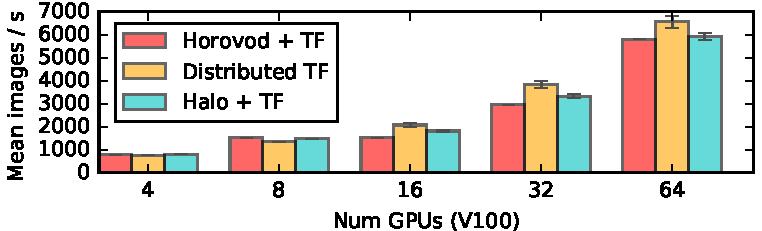
\includegraphics[width=3.1in,keepaspectratio]{fig/sgd_plot.pdf}
    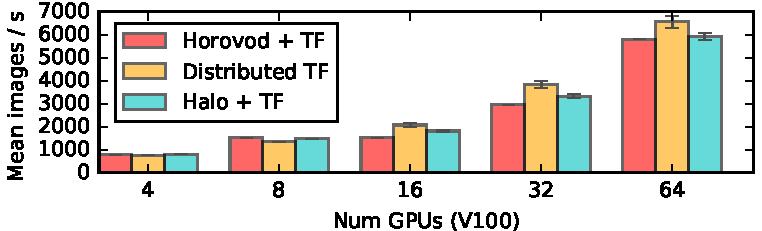
\includegraphics{fig/sgd_plot.pdf}
    \caption{
    \small{
        Images per second reached when distributing the training of a
        ResNet-101 TensorFlow model (from the official TF benchmark).
        %The \System{} implementation matches the performance of Horovod and
        %is within 10\% of distributed TensorFlow.
        All experiments were run on p3.16xl instances connected by 25Gbps Ethernet, and
        workers allocated 4 GPUs per node as done in Horovod~\cite{horovod}.
        We note some measurement deviations from previously reported, likely
        due to hardware differences and
        recent TensorFlow performance improvements. We used
        OpenMPI 3.0, TF 1.8, and NCCL2 for all runs. 
        {\color{red} TODO: replace Halo with Ray.}
    }
    }
    \label{fig:sgd}
\end{figure}

\begin{figure}
    \centering
    % 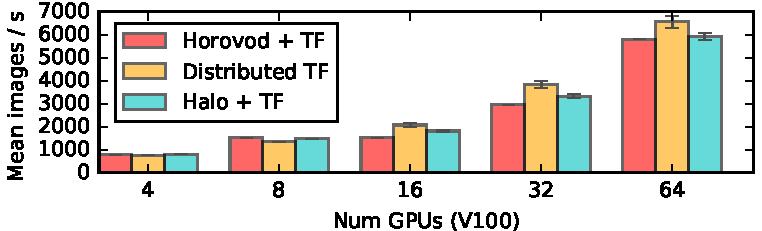
\includegraphics[width=3.1in,keepaspectratio]{fig/sgd_plot.pdf}
    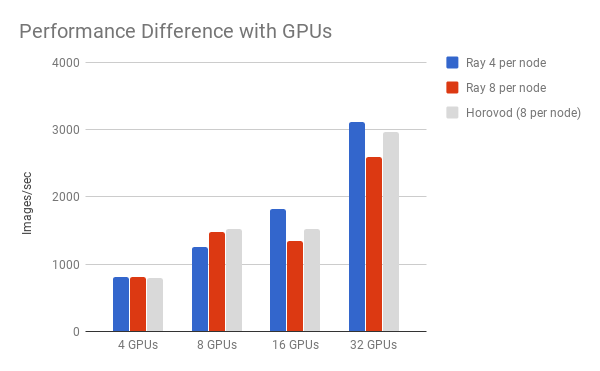
\includegraphics[width=3.1in,keepaspectratio]{fig/4to8.png}
    \caption{
    \small{
        Performance differences for using 4 GPUs per node vs 8 GPUs per node. In all cases, we use the same hardware (p3.16xlarge). However, we see there are performance differences going from 4 GPUs to 8 GPUs when comparing the number of GPUs per node. We provide Horovod performance for reference.
    }
    }
    \label{fig:8-vs-4-gpu}
\end{figure}

\begin{figure}
    \centering
    % 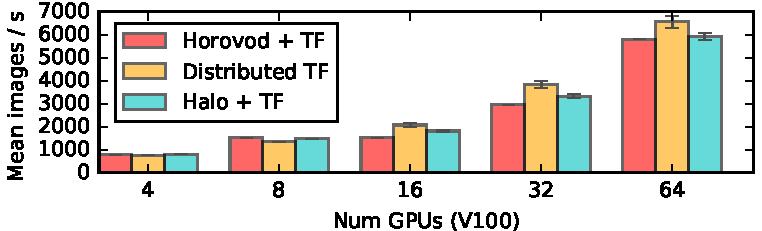
\includegraphics[width=3.1in,keepaspectratio]{fig/sgd_plot.pdf}
    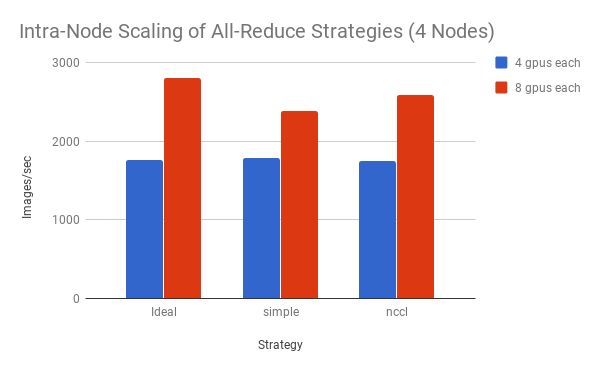
\includegraphics[width=3.1in,keepaspectratio]{fig/intranode.png}
    \caption{
    \small{
        Changing the all reduce strategy among GPUs within a node, and running a synchronous parameter server strategy between nodes. Ideal is generated by taking the gradient of the a single GPU, bypassing any communication overhead between GPUs on a single machine. "Simple" performance simply takes an average across all of the GPUs {\color{red} TODO: FIX THIS.}. "NCCL" performance uses the NCCL communication primitives to perform an all-reduce across the GPUs. We see that even though NCCL performance is better at 8 GPUs than "Simple", both provide sublinear scaling when doubling the number of GPUs per machine. 
    }
    }
    \label{fig:intra-node-allreduce-strategy}
\end{figure}


\section{Future Work}
{\color{red} TODO}


{
\footnotesize
\bibliographystyle{acm}
\bibliography{ray}
}

\end{document}
